% !TEX root = main.tex

\section{模型验证}
\subsection{线性时序逻辑}
\begin{definition}[线性时序逻辑(linear-time temporal logic, LTL)]
BNF定义如下
\[\phi::=\top\mid\bot\mid p\mid
(\lnot\phi)\mid
(\phi\land\phi)\mid
(\phi\lor\phi)\mid
(\phi\to\phi)\mid
(X\phi)\mid
(F\phi)\mid
(G\phi)\mid
(\phi U\phi)\mid
(\phi W\phi)\mid
(\phi R\phi)\]
其中$X,F,G,U,R,W$都称为时序连接词(temporal connectives)
\begin{itemize}
	\item $X$:neXt state
	\item $F$:some Future state(存在)
	\item $G$:all future states (Globally)(任意)
	\item $U$:Until(二元)
	\item $R$:Release(二元)
	\item $W$:Weak-until(二元)
\end{itemize}
运算符优先级
\begin{itemize}
	\item 一元连接词:$\lnot,X,F,G$
	\item $U,R,W$
	\item $\land,\lor$
	\item $\to$
\end{itemize}
\end{definition}
\begin{definition}[转移系统(transition system)]
一个转移系统$\mM=(S,\to,L)$是状态集合$S$(静态结构),转移关系$\to$(动态结构),使得$\forall s\in S,\exists s'\in S:\;s\to s'$,且有标注函数$L:S\to\mathcal{P}(Atoms)$,其中$\mP(Atoms)$为原子描述的幂集(实际上$L$就是给所有命题原子做真值指派)。
转移系统也可以被称作模型(model)。
\end{definition}
\begin{figure}[H]
\centering
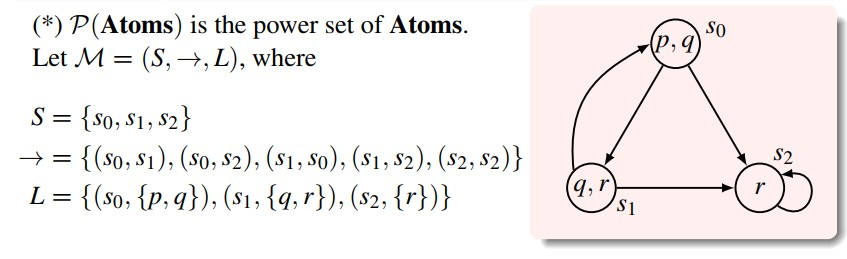
\includegraphics[width=0.8\linewidth]{fig/transition_system.jpg}
\end{figure}
\begin{definition}[路径(path)]
路径是一个无穷序列$s_1,s_2,\ldots\in S$使得$s_i\to s_{i+1},\forall i\geq 1$。
令$\pi^i=s_i\to s_{i+1}\to\cdots$为从状态$s_i$开始的路径。
路径$\pi=s_1\to s_2\to\cdots$满足LTL公式定义在满足关系$\models$上:
\begin{enumerate}
	\item $\pi\models\top$
	\item $\pi\not\models\bot$
	\item $\pi\models p$ iff $p\in L(s_1)$
	\item $\pi\models\lnot\phi$ iff $\pi\not\models\phi$
	\item $\pi\models\phi\land\psi$ iff $\pi\models\phi$ and $\pi\models\psi$
	\item $\pi\models\phi\lor\psi$ iff $\pi\models\phi$ or $\pi\models\psi$
	\item $\pi\models\phi\to\psi$ iff $\pi\models\psi$ when $\pi\models\phi$
	\item $\pi\models X\phi$ iff $\pi^2\models\phi$
	\item $\pi\models G\phi$ iff $\forall i\geq 1:\;\pi^i\models\phi$
	\item $\pi\models F\phi$ iff $\exists i\geq 1:\;\pi^i\models\phi$
	\item $\pi\models \phi U\psi$ iff $\exists i\geq 1:\;\pi^i\models\psi$ and $\forall j=1,\ldots,i-1:\;\pi^j\models\phi$
	\item $\pi\models \phi W\psi$ iff \textbf{either} $\exists i\geq 1:\;\pi^i\models\psi$ and $\forall j=1,\ldots,i-1:\;\pi^j\models\phi$ \textbf{or} $\forall k\geq 1:\;\pi^k\models\phi$
	\item $\pi\models \phi R\psi$ iff \textbf{either} $\exists i\geq 1:\;\pi^i\models\phi$ and $\forall j=1,\ldots,i:\;\pi^j\models\psi$ \textbf{or} $\forall k\geq 1:\;\pi^k\models\psi$
\end{enumerate}
记$\mM,s\models\phi$表示对于所有$\mM$开始于$s$的执行路径$\pi$,都有$\pi\models\phi$,或可简写为$s\models\phi$
\end{definition}
注意有以下恒等式
\[\begin{aligned}
\lnot G\phi&\equiv F\lnot\phi\\
\lnot F\phi&\equiv G\lnot\phi\\
\lnot X\phi&\equiv X\lnot\phi\\
\phi W\psi&\equiv \phi U\psi\lor G\phi\\
\phi R\psi&\equiv \lnot(\lnot\phi U\lnot\psi)\\
F(\phi\lor\psi)&\equiv F\phi\lor F\psi\\
G(\phi\land\psi)&\equiv G\phi\land G\psi\\
F\phi&\equiv\top U\phi\\
G\phi&\equiv\bot R\phi\\
\phi U\psi&\equiv\phi W\psi\land F\psi\\
\phi W\psi&\equiv\phi U\psi\lor G\phi\\
\phi W\psi&\equiv\psi R(\phi\lor\psi)\\
\phi R\psi&\equiv\psi W(\phi\land\psi)
\end{aligned}\]
\begin{example}
对于上图的例子,有以下式子成立
\begin{itemize}
	\item $s_0\models p\land q$ (3,5)
	\item $s_0\models X r$,因$r\in L(s_1),L(s_2)$
	\item $s_0\models G\lnot (p\land r)$,因所有从$s_0$开始的路径都满足$G\lnot(p\land r)$,也即满足$\lnot(p\land r)$
\end{itemize}
\end{example}

\subsection{模型检查}
下面是一个互斥锁的例子,$n$为非临界区状态,$t$为尝试进入临界区,$c$为临界区状态。
考虑2个进程,每个进程的转移都是$n\to t\to c\to n\to\cdots$。
\begin{figure}[H]
\centering
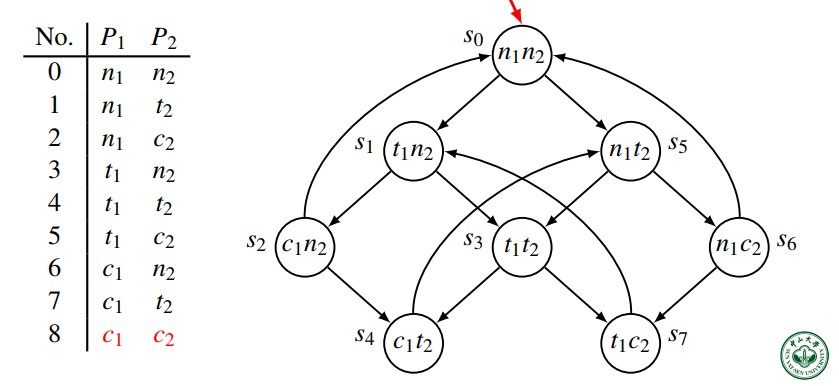
\includegraphics[width=0.8\linewidth]{fig/mutual_exclusion.jpg}
\end{figure}
有以下性质:
\begin{itemize}
	\item 安全性(safety):$G\lnot(c_1\land c_2)$在每个状态都被满足
	\item 活性(liveness):$G(t_1\to Fc_1)$,对于路径$s_0\to s_1\to s_3\to s_7\to s_1\to s_3\to\cdots$就不满足
	\item 非阻塞(non-blocking):对于任意状态满足$n_1$,有后继状态满足$t_1$,无法用LTL表达
	\item 非严格序列(strict sequencing)
\end{itemize}

\subsection{计算树逻辑}
\begin{definition}[计算树逻辑(computation tree logic, CTL)]
除了LTL有的$U,F,G,X$,CTL还有$A$和$E$表示\textbf{所有}路径(All path)和\textbf{存在}一条路径(Exist a path)。
BNF定义如下
\[\begin{aligned}
\phi::=&\top\mid\bot\mid p\mid
(\lnot\phi)\mid
(\phi\land\phi)\mid
(\phi\lor\phi)\mid
(\phi\to\phi)\mid
(AX\phi)\mid
(EX\phi)\mid\\
&(AF\phi)\mid
(EF\phi)\mid
(AG\phi)\mid
(EG\phi)\mid
A[\phi U\phi]\mid
E[\phi U\phi]
\end{aligned}\]
运算符优先级
\begin{itemize}
	\item $\lnot,AG,EG,AF,EF,AX,EX$
	\item $\land,\lor$
	\item $\to,AU,EU$
\end{itemize}
\end{definition}
\begin{definition}[CTL*]
$\phi$为状态公式(在状态上求值),$\alpha$为路经公式(在路径上求值)
\[\begin{aligned}
\phi&::=
\top\mid
p\mid
(\lnot\phi)\mid
(\phi\land\phi)\mid
A[\alpha]\mid
E[\alpha]\\
\alpha&::=\phi\mid
(\lnot\alpha)\mid
(\alpha\land\alpha)\mid
(\alpha U\alpha)\mid
(G\alpha)\mid
(F\alpha)\mid
(X\alpha)
\end{aligned}\]
\end{definition}
\begin{figure}[H]
\centering
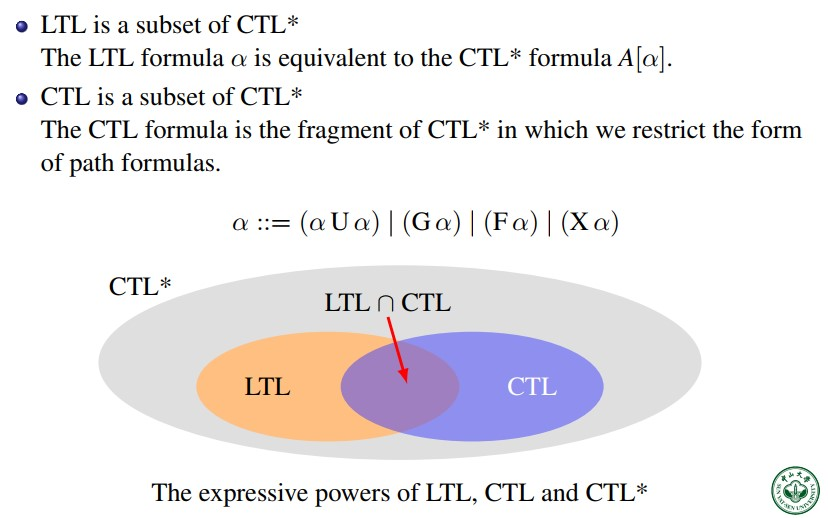
\includegraphics[width=0.8\linewidth]{fig/ltl_ctl.jpg}
\end{figure}